\documentclass[25pt, a0paper, portrait, blockverticalspace=.5cm]{tikzposter}
\usepackage[utf8]{inputenc}
\usepackage{amssymb,amsfonts,amsmath,mathtext,mathtools}
\usepackage{xfrac}
\usepackage{enumitem}

\let\vec\oldvec
\newcommand{\vec}[1]{\boldsymbol{#1}}

\title{\parbox{\linewidth}
	{\centering
		Acceleration and Crossing of Transition Energy Investigation Using an RF Structure of the Barrier Bucket Type in the NICA Accelerator Complex\		
}}
\author{S. KOLOKOLCHIKOV\textsuperscript{1}, Y. SENICHEV\textsuperscript{1}, E. SYRESIN\textsuperscript{2}, A. MELNIKOV\textsuperscript{1}}
\institute{
	\textsuperscript{1} Institute for Nuclear Research of the Russian Academy of Sciences, Moscow, Russia\\
	\textsuperscript{2} Joint Institute for Nuclear Researches, Dubna, Russia
}
\usetheme{Simple}
\usecolorstyle{Russia}
\colorlet{blocktitlefgcolor}{black}

\usepackage{caption}
\captionsetup{font=large}
\usepackage{multicol}
\setlength\columnsep{1.5cm}

\begin{document}

\maketitle

\block{INTRODUCTION}{
	\begin{multicols}{3}
\par During particle acceleration  to the energy of experiment $E_{exp}=12.6$ GeV ($\gamma_{exp}=14.4$) in NICA collider there is a need for the crossing of transition energy  $E_{tr}=5.709$ GeV ($\gamma_{tr}=7.087$). The slip-factor $\eta=\frac{1}{\gamma_{tr}^2}-\frac{1}{\gamma^2}$ , which included in the equation of longitudinal motion, changes the sign, that leads to a loss of stability in the longitudinal plane when $\gamma$ approaching to $\gamma_{tr}$. In order to minimize the reduction of the beam parameters, a rapid jump of transition energy is assumed during the time $t_{jump}\approx10$ ms [1] with a simultaneous change of the polarity of the RF system to ensure the stability of the beam after the jump. RF structure based on “Barrier Bucket” a feature of the NICA collider accelerating system. A non-zero value of the field between the barriers, ensures the acceleration of the beam. This feature makes the system original.
In this paper, the main features of the dynamics of the longitudinal motion of the beam crossing through the transition energy are considered, taking into account its jump in the RF structure of the “Barrier Bucket” type. Due to the rapid jump of transition energy the time at which the particles are near the zero value of the first order slip-factor is significantly reduced.  Obviously, in this case, the second order of the slip-factor begins to play a decisive role in the behaviour of particles inside the barrier bucket and completely determines the stability region near transition. In this case, when energy of particles crosses transition energy, focusing of the beam in the longitudinal plane disappears and the influence of the space charge becomes essential.
	\end{multicols}
	}

\begin{columns}
	\column{.5}
	\block{RAPID JUMP OF THE TRANSITION ENERGY}{
		\begin{minipage}{0.485\linewidth}
			\begin{tikzpicture}
			\node (cone) at (0,0) {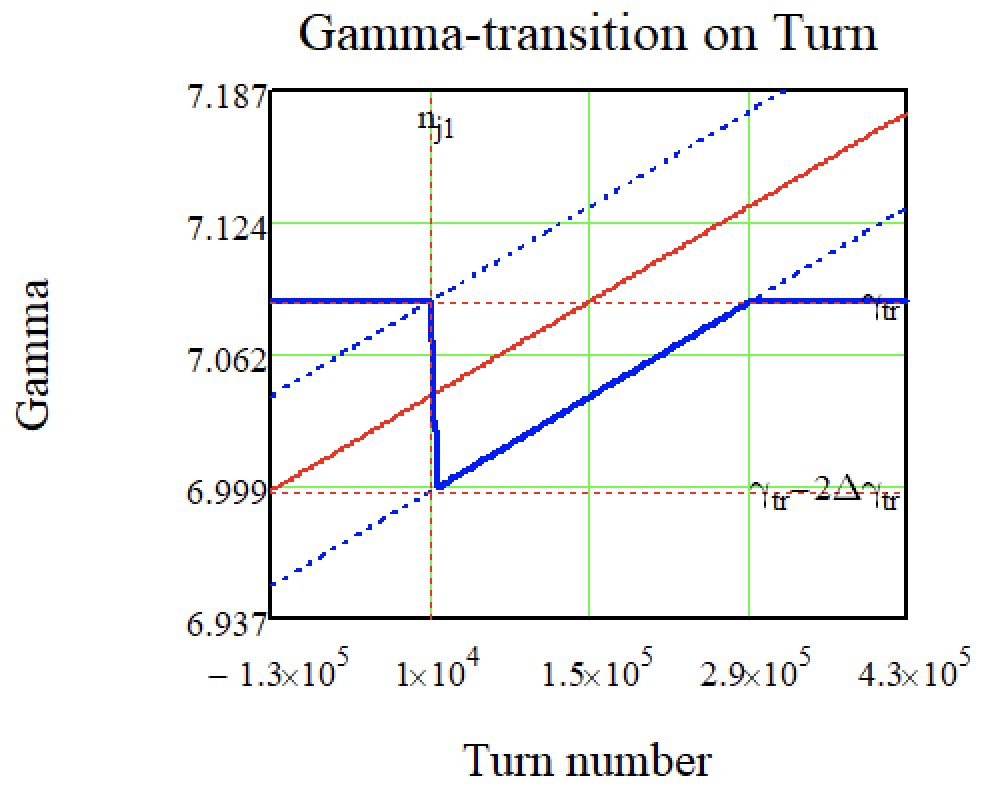
\includegraphics[width=\linewidth]{TEXPaper/img/WEPOPT004_f1-1.png}};
			\end{tikzpicture}
		\end{minipage}
		\begin{minipage}{0.485\linewidth}
			\begin{tikzpicture}
			\node (cone) at (0,0) {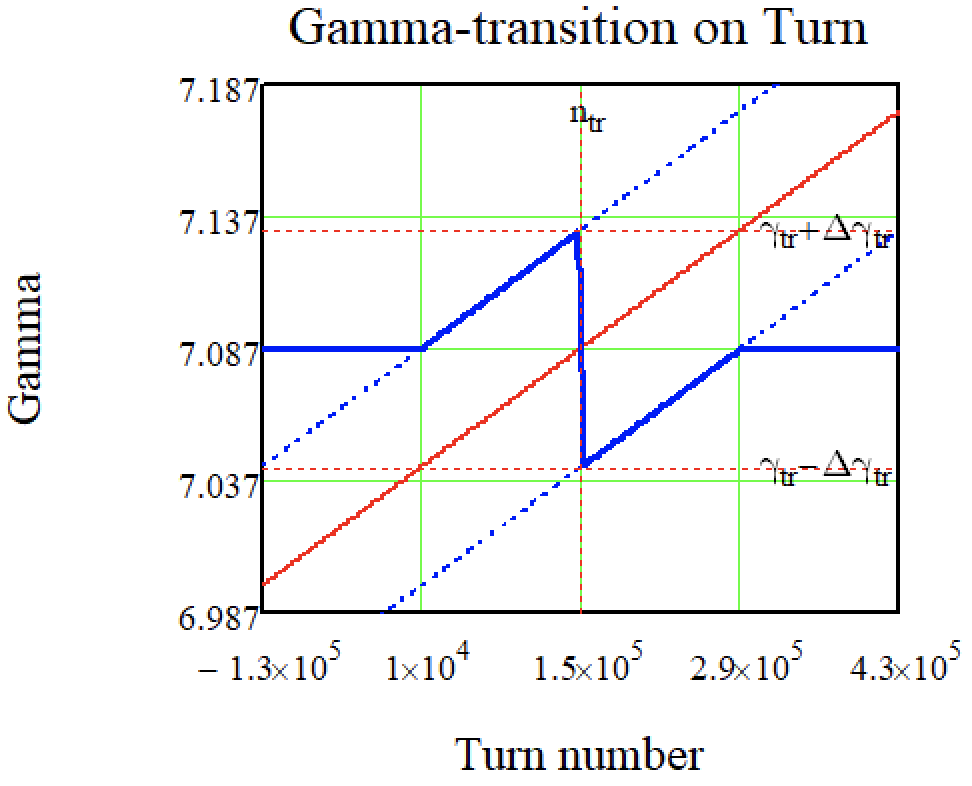
\includegraphics[width=\linewidth]{TEXPaper/img/WEPOPT004_f1-2.png}};
			\end{tikzpicture}
		\end{minipage}
		\par When the particle energy approaches the transition energy, it is assumed to make a rapid jump of transition energy. This can be achieved by changing the field gradient in the focusing quadrupoles of the arcs, since for periodic structures $1/\gamma_{tr}^{2}=\alpha_{0}=1/\nu_{x}^{2}$ [2], where $\alpha_{0}$ – first order of momentum compaction factor, $\nu_{x}$ – tune in the horizontal plane. The maximum change rate of transition energy is limited by the parameters of quadrupoles and their power systems $\dot\gamma_{tr}=\frac{d\gamma_{tr}}{dt}=8.5 s^{-1}$. Such a jump can be made during the time:
		\begin{equation}
		t_{jump}=T_{0} \Delta n_{jump}=\frac{2 \cdot \Delta \gamma_{tr}}{\dot{\gamma}_{tr}}=10.5 ms,
		\end{equation}
		\par where $T_{0}=1.7 \mu s$ – the time of one revolution period in the ring, $\Delta n_{jump}=6226$ – the number of revolution periods during transition.\\
		\par With the changed parameters of quadrupole lenses, the dynamic aperture was evaluated, it determines the stable area for movement of particles in the transverse plane. The corresponding calculations were carried out using OptiM and MADX programs [3].
	}	
	\block{BARRIER BUCKET RF SYSTEM}{
		\begin{minipage}{0.465\linewidth}
			\begin{tikzpicture}
			\node (cone) at (0,0) {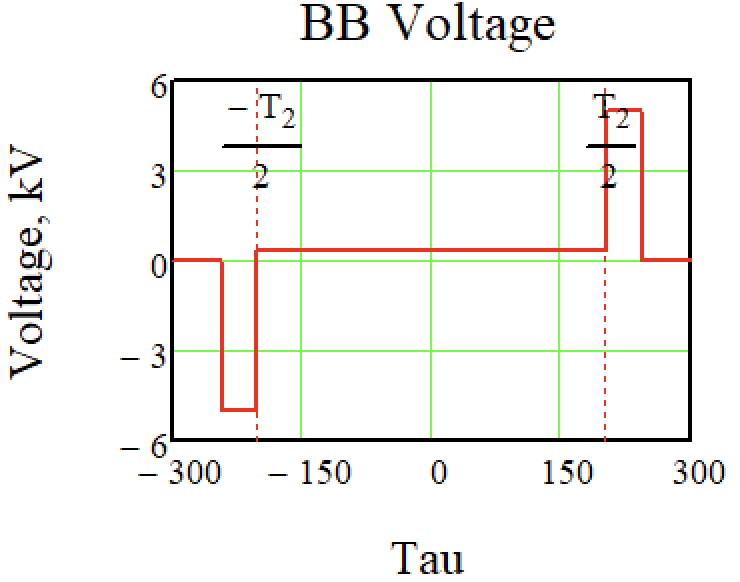
\includegraphics[width=\linewidth]{TEXPaper/img/WEPOPT004_f3-1.png}};
			\end{tikzpicture}
		\end{minipage}
		\begin{minipage}{0.495\linewidth}
			\begin{tikzpicture}
			\node (cone) at (0,0) {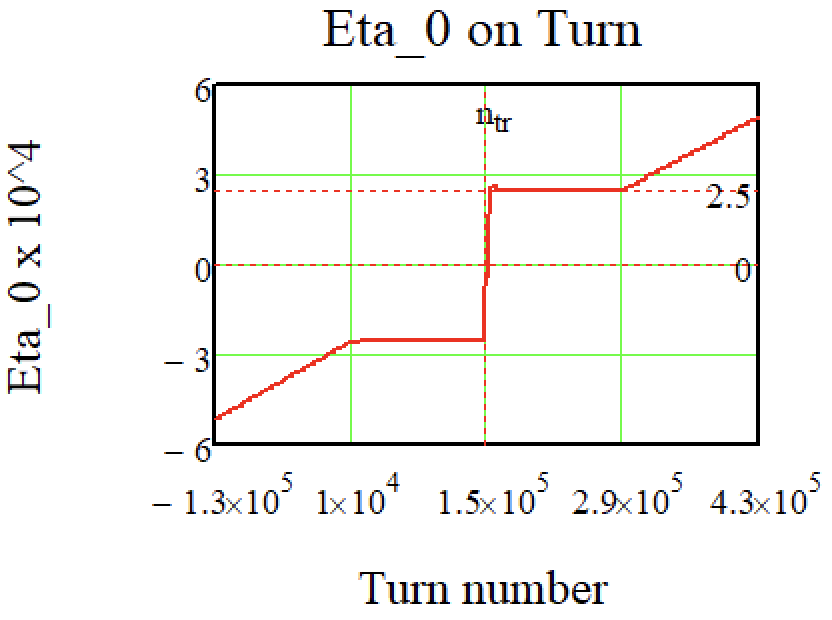
\includegraphics[width=\linewidth]{TEXPaper/img/WEPOPT004_f3-2.png}};
			\end{tikzpicture}
		\end{minipage}
		
\par The RF-1 system is used to retain, accumulate and accelerate particles to the experimental energy in the collider rings. Each collider ring has one RF-1 system. During retention and accumulation, 2 pairs of rectangular pulses with opposite signs are generated with the amplitude of each barrier $V_{bb}=\pm5$ kV. The time duration of a single pulse can vary from $T_{bb}=10$ till $80$ ns. The accumulated particles enclosed between 2 pulses will be inductively accelerated by a constant potential $V_{acc}=300$ V [1]. \\

\par When the energy approaches the transition value, the RF barriers turn off and, after the proton energy becomes greater, the RF barriers turn on and a polarity changes. This is necessary because the slip-factor value changes it’s sign after crossing. Before the jump itself, due to the symmetry with respect to zero, it will be equal to the value after:
$$
\left|-\eta_{0 t r}\right|=\left|+\eta_{0 t r}\right|=\left|\eta_{0}\left(\gamma_{t r}-\Delta \gamma_{t r}\right)\right|=2.5 \cdot 10^{-4}
$$

	}
	
	\column{.5}
	\block{LONGITUDINAL DYNAMIC}{
	
		\begin{minipage}{0.40\linewidth}
			\begin{tikzpicture}
			\node (cone) at (0,0) {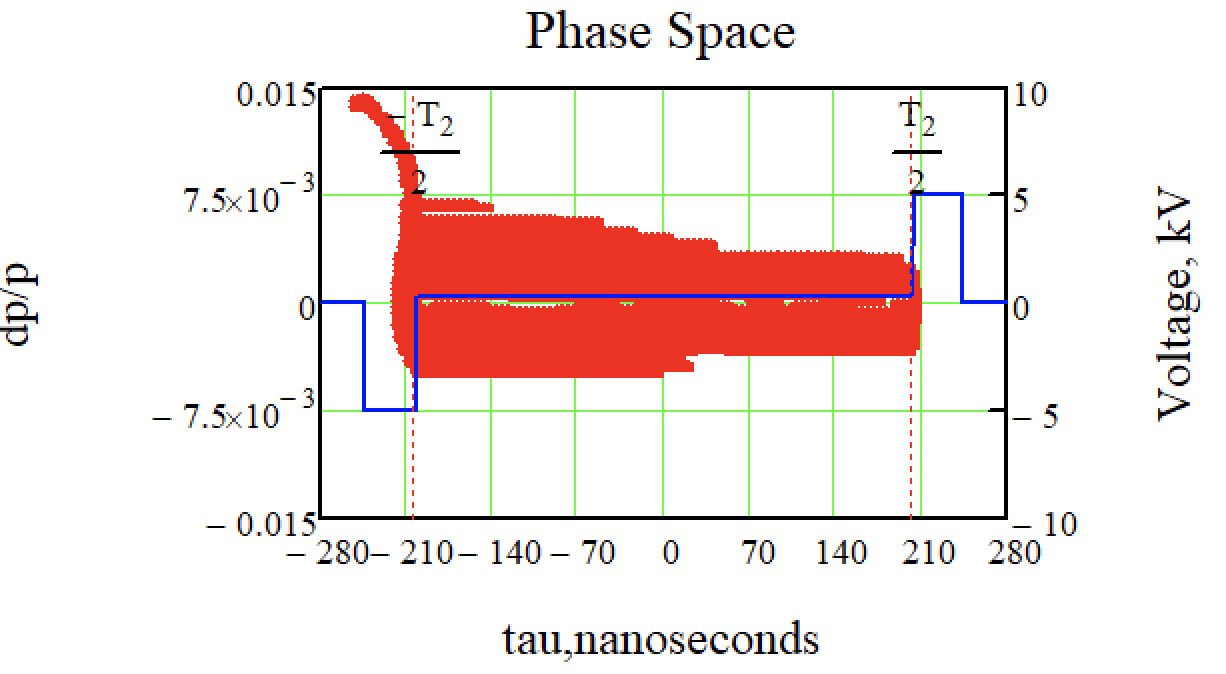
\includegraphics[width=\linewidth]{TEXPaper/img/WEPOPT004_f4-1.png}};
			\end{tikzpicture}
		\end{minipage}
		\begin{minipage}{0.29\linewidth}
			\begin{tikzpicture}
			\node (cone) at (0,0) {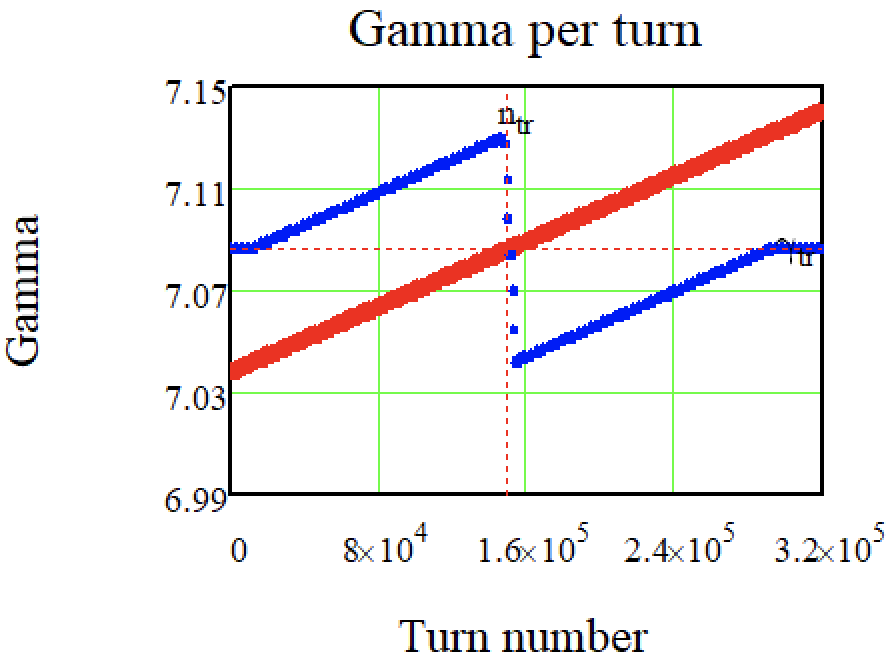
\includegraphics[width=\linewidth]{TEXPaper/img/WEPOPT004_f4-2.png}};
			\end{tikzpicture}
		\end{minipage}
		\begin{minipage}{0.28\linewidth}
			\begin{tikzpicture}
			\node (cone) at (0,0) {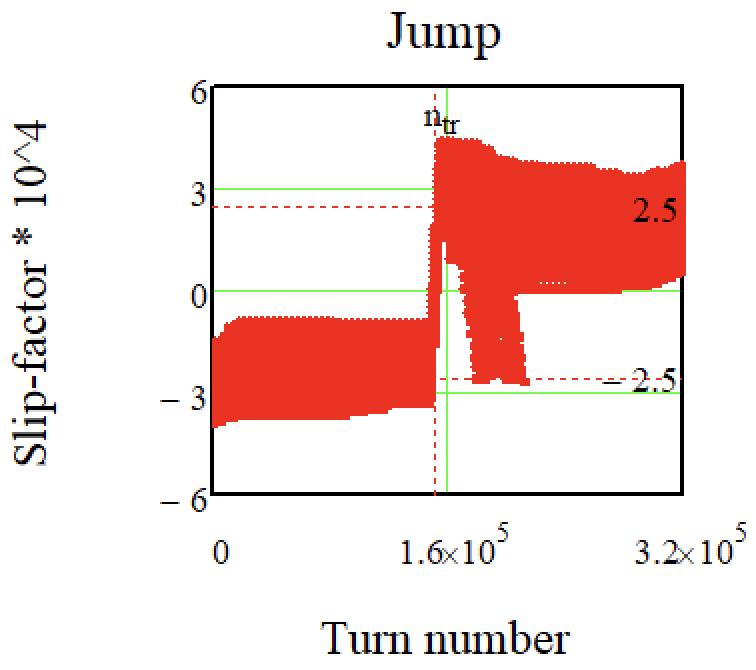
\includegraphics[width=\linewidth]{TEXPaper/img/WEPOPT004_f4-3.png}};
			\end{tikzpicture}
		\end{minipage}
		
		\par Equations of longitudinal motion in Barrier Bucket in coordinates ($\tau$,$\Delta E$) [4]: 
		
		\begin{equation}
		\frac{d \tau}{dt}=\frac{\eta h}{\beta^{2} E_{0}} \Delta E \quad \text { and } \quad \frac{d \Delta E}{dt}=\frac{Ze}{A} \frac{\omega_{0}}{2 \pi} U g(\tau)
		\end{equation}

\par where $E_0$ – synchronous particle energy, $Ug(\tau)$ – voltage generated by RF-barriers, $\omega_{0}=2\pi/T_{0}$ , $h$ – harmonic number.\\
		
\par There is a jump of slip-factor in a different time for different particles because of dependence of slip-factor on $\delta$. Obviously, after the jump, particles with a negative value of the slip-factor will not be in a stable region, since the polarity of the retaining barriers changes and will tend to leave the phase plane. Also, due to the momentum spread, there is an asymmetry of the phase portrait relate to the zero value of the momentum spread $dp/p$.\\
		
\par Before the jump ($\eta_{0}<0$) particles with negative $\delta<0$ have a slip-factor value $\eta$ closer to zero than particles with positive $\delta>0$. Because of this, the phase plane behaves asymmetrically, since the total value of the slip-factor affects the dynamics and change coordinate $\tau$. Thus, the particles accumulate in the area of the left barrier. During the jump, the RF is turned off and does not affect the dynamics. After the jump ($\eta_{0}>0$) the particle distribution is shifted to the left edge and now the opposite is true – for particles with positive $\delta>0$ the value of the slip-factor $\eta$ is closer to zero, than for particles with $\delta<0$. Those particles that turned out to be on the left in the area of the RF barrier (with reversed polarity) due to the proximity to the zero value of the slip-factor, do not have time to stay in the separatrix.

		
	}
	\block{CONCLUSION}{
	\par During modelling and calculations, it was found that with a transition energy jump, the determining factor, which influence on the stability of the particles inside the Barrier Bucket RF system is the second order of slip-factor. It depends on momentum spread and can determine the maximum momentum spread for the transition energy crossing in a jump-scheme without loss. Also, it is necessary to take into account the space charge and impedances. These problems require further research.

	}
	\block{REFERENCES}{
	 
	\par [1] Syresin, E. M., Butenko, A. V., Zenkevich, P. R., Kolokolchikov, S. D., Kostromin, S. A., Meshkov, I. N., Mityanina, N. V., Senichev, Y. V., Sidorin, A. O., Trubnikov, G. V. (2021). Formation of Polarized Proton Beams in the NICA Collider-Accelerator Complex. Physics of Particles and Nuclei, 52(5), 997-1017.https://doi.org/10.1134/S1063779621050051
	\par [2] K. Y. Ng. Physics of Intensity Dependent Beam Instabilities. Fermilab-FN-0713(2002).
	\par [3] F. Schmidt,P. Skowronski,V. Lebedev,A. Valishev. Higher Order Dispersion and Momentum Compaction in MAD-X/PTC using NormalForm.CERN-ACC-NOTE-2018-006
	\par [4] Hans Stockhorst, Takeshi Katayama, Rudolf Maier. Beam Cooling at COSY and HESR Theory and Simulation – Part 1 Theory. Forschungszentrum Jülich GmbH Zentralbibliothek, Verlag Jülich. ISBN 978-3-95806-127-9(2016) p161-171.
	}
	
\end{columns}


\begin{columns}



\end{columns}

\end{document}